For the refresh strategy defined in BMI, the BASH system works reasonably well.
However, its inefficiencies become more significant as we design refresh
strategies which require more computation. While the original
implementation is suitable for simulation purposes, it is inefficient and
difficult to use in a real world use-case.
As part of our TREC 2017 Core effort, we designed a CAL-powered review tool
called HiCAL. We intended this tool to process relevance feedback as soon as
possible (in other words, more frequent refreshes). For a smooth user
experience, we wanted to achieve this with minimum possible system delay. Due to
to these reasons, we decided to implement CAL from scratch in C++. We chose C++
because it provides a good control over efficiency and is usually easy to
maintain/extend.
We wanted to build a system which along with satisfying all the requirements of
HiCAL, could be easily used for other applications and future research, such as
the work presented in this thesis. We designed this system to meet the following
goals:
\begin{itemize}
\item Fast and efficient.
\item Support parallel tasks (useful for supporting parallel simulations and
multiple users).
\item Easy to use as a standalone tool or as a part of an external application.
\item Easy to extend and modify any step of the CAL algorithm.
\end{itemize}
\subsection{Design}
In this section, we briefly discuss the design details of our CAL
ystem.
Prior to using CAL system, a one-time preprocessing step is required to convert a
given text collection to machine readable set of feature vectors. The corpus
processor takes as input an archive (a tar.gz file) of text documents, computes
the feature vectors for every document, and writes them to a binary file. We use
binary files over human-readable text files to significantly improve the output
file size and loading times. \red{Provide numbers to quantify the difference}
Each document is assigned an ID which is its filename (ignoring the directory
structure) in the input archive. This ID is used to judge and retrieve documents
in the CAL system. The files are treated as plaintext files and are assumed to
be cleaned as per the needs of the user. Figure~\ref{fig:preprocessing} shows
a preprocessing pipeline example with New York Times collection.  By default, the
corpus preprocessor computes tf-idf unigram features for every documents as
explained in the previous chapter.
\begin{figure}[h]
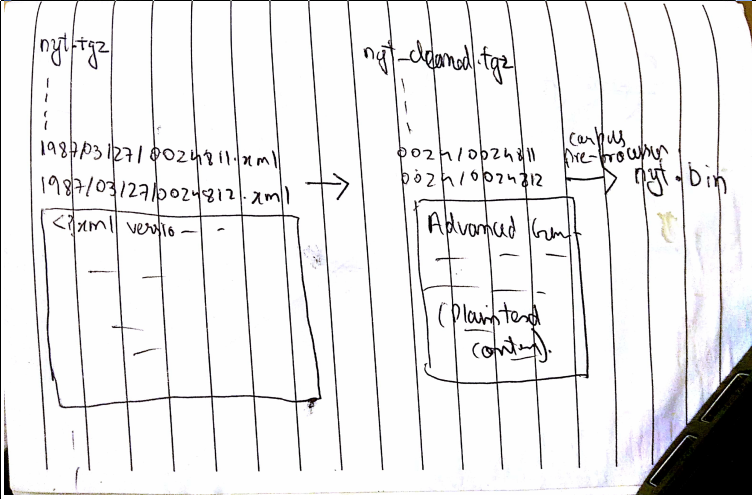
\includegraphics[width=\textwidth]{tmp_pictures/preprocessing_pipeline.png}
\caption{Preprocessing pipeline for New York Times collection}
\label{fig:preprocessing}
\end{figure}
The output binary file contains document frequency data followed by the document
feature data. The binary file format is described in
Figure~\ref{fig:binary_format}.
\begin{figure}[h]
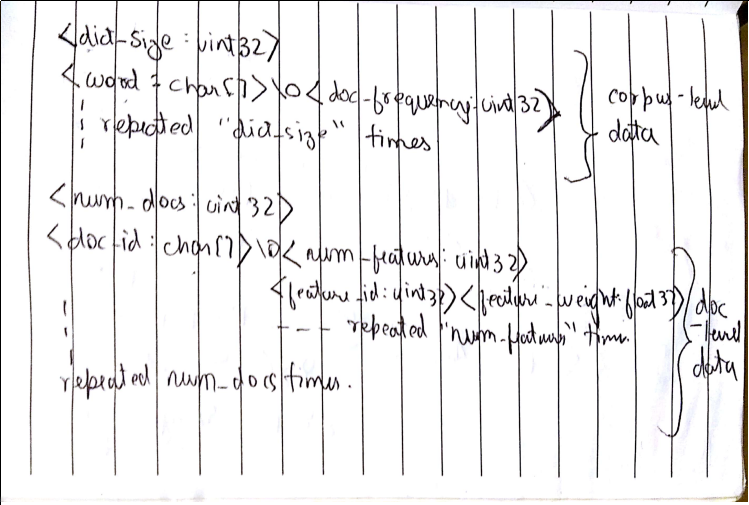
\includegraphics[width=\textwidth]{tmp_pictures/binary.png}
\caption{Description of the binary file outputted by the corpus preprocessor}
\label{fig:binary_format}
\end{figure}
The CAL system takes as input the corpus features (the binary output file
of the corpus preprocessor) and loads it in the memory. The document feature
vectors are kept in the memory throughout the lifetime of a CAL process in order
to ensure fast operations and reduce disk access. A review task is initiated by
a seed query string provided by the user. The user can also specify
seed document judgments and the choice of refresh strategy. The system handles
these tasks concurrently, so that multiple users can review documents
at the same time.
There are two ways to interact with the CAL system. The command line tool can be
used for testing and simulation purposes. The more robust and user-friendly HTTP
API should be used for most purposes.
